\chapter{Introduction}
\label{chap:introduction}

\section{Initial Situation}
Digital Twins (DT) are a key technology at the front of the fourth industrial revolution, often referred to as Industry 4.0.
The latter term is characterized by the integration of cyber-physical systems (CPS), the Internet of Things (IoT), and cloud computing to create smart factories aimed at automation and efficiency \autocite{Oztemel2020}. Companies pursue this vision by trying to remain competitive through the adoption of innovative technologies that promise enhanced productivity and reduced operational costs. One such technology that supports this transformation is the DT. It can be defined as a virtual representation of physical assets enabling real-time monitoring and optimization \autocite{Tao2018ijamt}. The DT bridges the connection between the two entities with a bi-directional data flow to exchange information and to influence the behavior of the physical asset \autocite{grieves2014digital}. This technology is central to Industry 4.0, facilitating the physical and digital worlds through real-time data integration, simulation, and optimization \autocite{judijanto2024trends}.

Although this discipline is rapidly evolving, a unified definition of DT has yet to be established due to the diverse requirements and perspectives across different fields. In engineering, the focus might be on the real-time interaction between physical systems and their digital counterparts, whereas in computer science, the emphasis is often on data integration and simulation capabilities. These varying priorities result in multiple interpretations and applications of the term DT. The concept was first introduced by Michael Grieves in 2002, who defined it as a digital representation of a physical object or system \autocite{grieves2014digital}. However, the concept has evolved since, encompassing a broader range of applications and technologies. In the literature, three termes are used to describe similar characteristics of DT: Digital Model (DM), Digital Shadow (DS), and Digital Twin (DT), see \Cref{fig:Kritzinger} \autocite{jones2020characterising,Zhang2021jmsy}.

\begin{figure}[htbp]
  \centering
  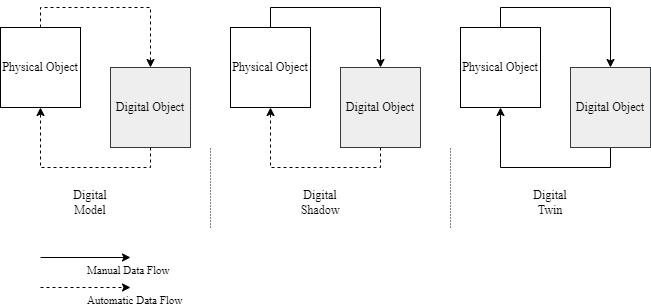
\includegraphics[width=0.8\textwidth]{figures/kritzinger.png}
  \caption{Comparison of Digital Shadow (DS), Digital Model (DM) and Digital Twin (DT) as presented by Kritzinger (2018). This distinction is crucial for understanding validation requirements across different digital representation types.}
  \label{fig:Kritzinger}
\end{figure}

The Digital Model (DM) represents the most basic form. It involves manual data connections between physical and digital entities. These connections can be temporarily shifted or even disconnected. There is no direct control of the digital object over the physical entity. It is primarily a simple or complex model \textit{describing} the physical object. The data flow must be manually triggered by the modeler, who also interprets the results and controls the DM.
The Digital Shadow (DS) is a more advanced version of the DM. It is a digital representation of the physical object that is continuously updated with real-time data, allowing for monitoring, analysis and simulation. While it can predict future states of the physical object based on the current state and historical data, it is not able to influence the physical object without human intervention. The control is, similar to the DM, still in the hands of the modeller. A DS is frequently used for simulation purposes and is sometimes misclassified as a DT in the literature \autocite{kritzinger2018digital,sepasgozar2021differentiating}.
The Digital Twin (DT) is the most advanced version of the three, offering a digital representation of the physical object, which is also continuously updated with real-time data. The DT can be used for monitoring, analysis, and \textit{control} purposes. It can predict the future states of the physical object based on the current state and historical data. The DT can also influence the physical object by sending control signals to it. The control is partially or completely in the hands of the DT. The DT thus \textit{can} serve more purpose than modelling or simulating the physical object. It may serve as an autonomous system, updating itself or with minimal human intervention \autocite{kritzinger2018digital}.

DTs are applied across various sectors, including manufacturing, defense, automotive, service, finance and healthcare \autocite{Tao2018ijamt}. Manufacturing is particularly notabl due to its high potential for process optimization and automation. This thesis focuses on the latter, particularly discrete material flow systems (DMFS). These systems process discrete objects (parts) moving along transportation routes or conveyor lines at regular or irregular intervals, integrating both production and logistics operations \autocite{arnold2005materialfluss, schwede2024learning}. A key simplification in their modeling is the abstraction of material flow as a sequence of discrete events, following the principles of discrete-event simulation (DES) \autocite{kovacs2016mathematical, robinson2014simulation}. DES is well-suited for analyzing complex systems where state changes occur at discrete points in time, such as arrivals, departures, and processing steps \autocite{robinson2014simulation}.

Historically, DM played a crucial role in the design, planning, and control of DMFS, primarily through applications like material flow simulations, logistic assistance systems, and digital factory implementations \autocite{Thiede2013}. However, advancements in both DS and DT have enabled a shift from isolated, use-case-specific models toward complete digital representations that span the entire lifecycle of DMFS \autocite{Abdoune2023}. This transition is largely driven by the growing demand for predictive capabilities by stakeholders and automated decision support in manufacturing systems, reflecting the core principles of Industry 4.0 \autocite{frank2019industry}. A second driver of DT innovation lies in the widely available data from IoT devices and sensors, which enhances model training and real-time adaptation of DTs \autocite{Tao2018ijamt}.

In practice, the automated data transfer between the digital model and the physical system is not always critical for DMFS management. Unlike in time-sensitive applications, human decision-makers often remain integral to the control loop, meaning that real-time automation is not always necessary \autocite{schwede2024learning}. Therefore, for this thesis, DS and DTs will be treated as equivalent concepts.

Beyond replicating the current state and managing historical data, DTs are essential for predicting system behavior and evaluating potential modifications. The widespread use of DES within digital twins highlights the central role of simulation-based DTs (SBDTs) in DMFS \autocite{Lugaresi2021aifac}. As \citeauthor{schwede2024learning} emphasize, SBDTs provide decision support for optimizing costs and performance in highly competitive manufacturing environments. While current SBDTs are primarily developed and updated manually by domain experts, emerging research explores how machine learning (ML) can enhance predictive accuracy and automate model updates by automatically learning model characteristics, reducing costs and development time.

Thus, the progression from digital models to simulation-based DTs reflects an ongoing shift toward data-driven, predictive, and increasingly automated representations of DMFS, enabling more informed decision-making throughout the system's lifecycle \autocite{boschert2016digital,lim2020state}.

\section{Problem}
Despite the transformative potential of DTs, their implementation can be challenging. Creating and maintaining accurate DTs require substantial investments in technology and domain knowledge. This investment is wasted if the resulting model fails to accurately represent the physical entity or produces incorrect results. While automatic generation may seem like an elegant solution, it carries risks such as overfitting or biased predictions \autocite{gemanbias}. Manufacturing data for training must be rigorously cleaned and preprocessed. Automatically generated DTs must also undergo automatic Validation, Verification, and Uncertainty Quantification (VVUQ) to preserve their cost and time advantages. Manual VVUQ, which relies on humans in the loop, hinders scalability, automatic synchronization with the physical entity, and depends on costly domain knowledge often provided by experts \autocite{Bitencourt2023}. These hurdles are significant barriers to automatic learning \autocite{ribeiro2016should,zhao2024data}. As industries integrate DT into their production processes, establishing trust becomes fundamental as well \autocite{trauer2022digital,arrieta2020explainable}. For widespread acceptance among coworkers, stakeholders, and investors, automatic DT creation and VVUQ must demonstrate clear advantages over manual creation and expert-led VVUQ.

Even when DT learning is successfully performed, questions about its correctness, precision, and robustness persist. These concerns are addressed by validation, verification, and uncertainty quantification frameworks (VVUQ) \autocite{sel2025survey}. Ensuring the validity, reliability, and accuracy of a DT is critical, yet traditional VVUQ approaches rely heavily on manual expert involvement and case-specific reference values \autocite{Bitencourt2023,hua2022validation}. This leads to inefficiencies, particularly in the context of automated DT generation, where such manual processes undermine the goal of reducing development effort. \citeauthor{hua2022validation} even argue that there are no robust and standardized verification and validation methods for DTs. As \autocite{sel2025survey} point out, uncertainty quantification is often overlooked, but addresses an important aspect of assessing low noise in explanations. One hurdle to standardized VVUQ frameworks is the lack of a clear definitions for validity and verification in the context of DTs \autocite{Bitencourt2023}.

For discrete material flow systems (DMFS), these challenges are even more pressing due to their procedural nature and inherent stochasticity. Rigorous VVUQ is essential to address the risk of manufacturing process failures caused by anomalies, resource constraints, software faults, or human error. This necessity arises because such failures can disrupt the intricate workflows and unpredictable dynamics inherent in DMFS, making reliable performance prediction a priority. When DTs for these systems are generated automatically, traditional validation methods become problematic, as they negate much of the efficiency gains through automation. This creates a fundamental conflict: while automated DT generation reduces initial development and updating efforts, it simultaneously increases the complexity of validation and verification, potentially counteracting its intended efficiency gains.

\section{Objective}

This thesis addresses this conflict by developing a data-driven framework for automated VVUQ of automatically generated, simulation-based DTs which have been learned from data. The focus lies on DMFS due to their practical relevance and dynamical, procedural nature. The research can further be specified by the following research questions (RQ):

\begin{itemize}
  \item \textbf{RQ1:} How can automated validation and verification processes for DTs be efficiently implemented to maintain accuracy?
  \item \textbf{RQ2:} Which data-driven approaches are best suited to identify discrepancies between simulated behavior and real operational data in discrete material flow systems?
  \item \textbf{RQ3:} To what extent does the developed framework improve the quality and reliability of DTs compared to traditional V&V methods?
\end{itemize}

This thesis proposes that object-centric event logs—commonly used to generate DTs in manufacturing—can also serve as the foundation for an automated, use-case-independent validation and verification framework. Such an approach would preserve the efficiency benefits of automated generation while ensuring that the resulting DTs meet necessary standards. A key aspect of this approach is the development and monitoring of generic, statistically grounded reference values, which must be quantifiable and have an underlying distribution. The framework will be evaluated using a case study from the discrete material flow domain, providing empirical evidence of its effectiveness in improving model accuracy and efficiency.

\section{Structure and Methodology}

\subsection*{Structure}
The thesis is organized into eight chapters.
\Cref{chap:theory} establishes the theoretical foundation. It begins with broad, domain-specific concepts and progressively narrows the focus to the core topics of this thesis: Automated verification and validation (VVUQ) of simulation-based digital twins (SBDTs) in discrete material flow systems.
\Cref{sec:material-flow} introduces material flow planning and simulation, outlining the key elements of production systems, such as processes, resources, and control mechanisms. It also defines key performance indicators (KPIs), essential for evaluating both real and simulated systems, providing the practical context in which DTs operate.
\Cref{sec:digital-twin} then transitions to the DT concepts. A framework for comparing DTs by \textcite{schwede2024learning} is presented. Special attention is given to data-driven DTs and their subset, automatically generated digital twins (AGDTs). The section concludes by contrasting AGDTs with classical simulation models, highlighting the challenges posed by automatically generated models.
Building on this foundation, \Cref{sec:process-mining} presents the principles of process mining (PM) and event log analysis, focusing on object-centric event logs as a data basis for automated validation. This section demonstrates how PM acts as a bridge between real-world process data and model validation, thus enabling continuous verification of SBDTs.
\Cref{sec:vvuq-sbdt} narrows the focus further to VVUQ in the context of SBDTs, beginning with a historical overview of VVUQ methodologies. It then addresses the specific challenges posed by automatically generated models, such as data dependency and lack of transparency in model creation. The section introduces machine learning-based approaches for VVUQ, particularly classification methods for detecting model deviation. It also explores the current state of VVUQ in corporate practice, emphasizing the need for continuous and automated validation processes.

\Cref{chap:methodology} outlines the methodology for developing the proposed framework. It begins with a requirements analysis, deriving functional, technical, and data format requirements from theoretical findings. The chapter then elaborates on the data-based validation strategy, machine learning-based validation approach, metrics for model evaluation, and online validation with continuous monitoring.

\Cref{chap:implementation} presents the implementation of the framework, starting with the architecture and system setup, followed by detailed descriptions of event log processing, simulation integration, and the machine learning pipeline.

\Cref{chap:case-study} presents the case study results, evaluating the framework's effectiveness in improving DT quality. It describes the application scenario and data basis, the automatically generated DT, validation experiments, and result interpretation. It concludes with a comparison to manual validation methods.

\Cref{chap:discussion} discusses the implications of the results and provides recommendations for future research. It evaluates the framework in light of the research questions, examines the significance of verification in automatically generated DTs, addresses limitations, and explores implications for research and practice.

\Cref{chap:conclusion} concludes the thesis by summarizing key findings and their implications. It addresses the research questions and hypotheses, discusses the significance of the results, acknowledges limitations, and provides recommendations for future work.

\subsection*{Methodology}

The thesis follows a Design Science Research approach (DSR). This approach is characterized by the development of artifacts to solve practical problems \autocite{hevner2004design,peffers2007design}. Artifacts in the sense of DSR are created objects or constructs which address the given problem and contribute to both theory and practice. The artifacts are evaluated in a real-world context to demonstrate their effectiveness. The thesis applies the cyclical DSR model, see figure \ref{fig:DSR}.

\begin{figure}[htbp]
  \centering
  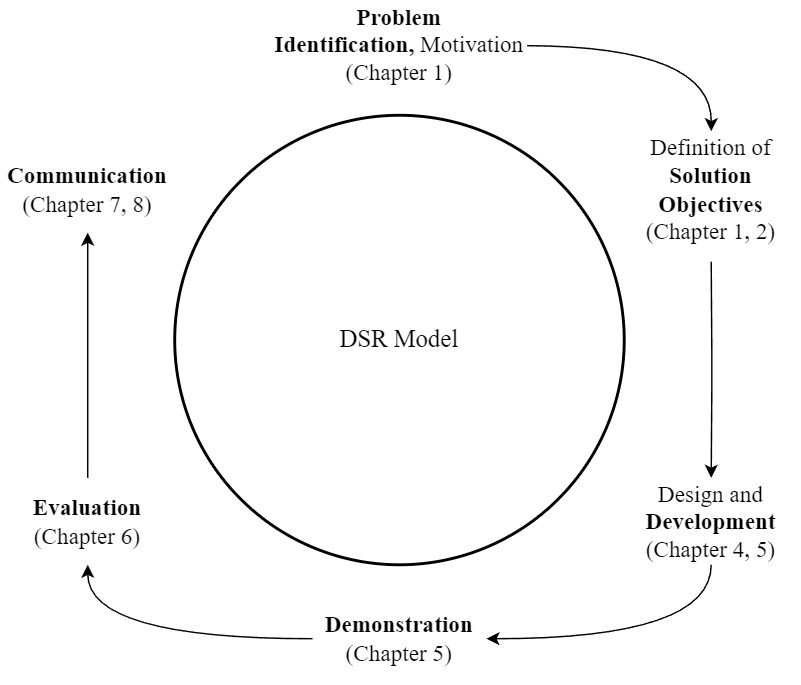
\includegraphics[width=0.8\textwidth]{figures/dsr.png}
  \caption{The cyclical design science research model. The model consists of six steps. The problem identification (1) refers to the research gap in automated VVUQ of SBDT. Defining the solution objectives (2) specifies the research gap by formulating questions and hypotheses based on the theoretical foundations. The design and development (3) phase includes the development of the framework. The demonstration (4) phase shows the application of the framework in a case study. The evaluation (5) phase assesses the effectiveness of the framework. The communication (6) phase concludes the research by presenting the results.}
  \label{fig:DSR}
\end{figure}

The research paradigm of the thesis is deductive-theory critical \autocite{eberhard1987einfuhrung}. A conceptual VVUQ framework is developed based on existing theoretical foundations, while deriving new requirements through a requirements analysis. The framework is then applied in a case study to evaluate its effectiveness. The research is critical in that it aims to improve the efficiency and effectiveness of VVUQ for automatically generated DTs. Elements of empirical research are included through the case study and the data-driven approach.

